\documentclass{article}
\usepackage{geometry}
\usepackage{listings}
\usepackage{color}
\usepackage{hyperref}
\usepackage{listings}
\usepackage{graphicx}
\usepackage{float}
\usepackage{sectsty}
\usepackage{enumitem}

\definecolor{codebackground}{rgb}{0.99,0.99,0.97}
\definecolor{mygray}{rgb}{0.5,0.5,0.5}

\lstset{
    basicstyle=\ttfamily,
    backgroundcolor=\color{mygray},
    keywordstyle=\color{blue},
    commentstyle=\color{mygray},
    showstringspaces=false,
    numbers=left,
    numberstyle=\tiny,
    numbersep=5pt,
    breaklines=true,
    frame=single,
    breakatwhitespace=false,
}

\geometry{a4paper, margin=0.75in}

\title{\textbf{\LARGE Homework 4 - Cache Experiments}\\[2ex] \large CS2323 - Computer Architecture, Autumn 2023}
\author{\textbf{\large{Soham Rajesh Pawar}}\\ CS22BTECH11055}
\date{November 9, 2023}

% Adjust section font sizes
\sectionfont{\LARGE}
\subsectionfont{\Large}

\begin{document}
\maketitle

\section{Question 1 :}
\textbf{\large{
Cache reads: Execute the assembly programs 1 and 2 and observe the hit rates for various data cache configurations.
You should vary the configurations atleast as per the following (you are free to explore more combinations as well):
Lines: 1, 2, 3 keeping Blocks as 2 and Ways as 0. In RIPES, Lines refers to the block size
Blocks: 3, 4, 5 keping Lines as 3 and Ways as 0. In RIPES, Blocks refers to the number of blocks
Ways: 0, 1 keeping Blocks as 2 and Lines as 3. In RIPES, Ways refers to the associativity.
}}
\subsection{Variation with Lines :}
\begin{figure}[H]
  \centering
  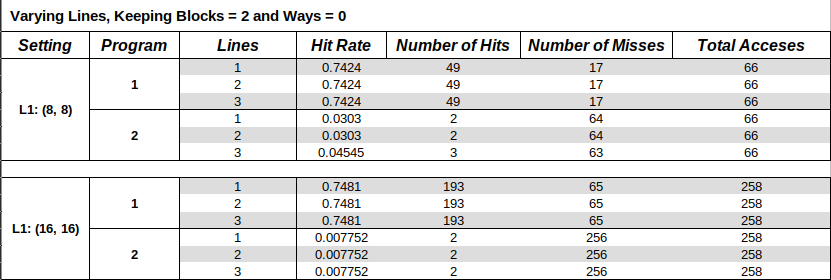
\includegraphics[width=1\textwidth]{1.1.png}
  %\caption{\large Performance Parameters}
  \label{fig:example}
\end{figure}
\noindent
\textbf{\large{Inference :}}\\
\begin{enumerate}[label=\alph*)]
  \item Program 1: The number of lines doesn't significantly impact the hit rate. This is because the memory access is contiguous increasing spatial locality.
  \item Program 2: A slight impact is observed on the hit rate, reducing the number of collisions.
\end{enumerate}
\smallskip

\subsection{Variation with Blocks :}
\begin{figure}[H]
  \centering
  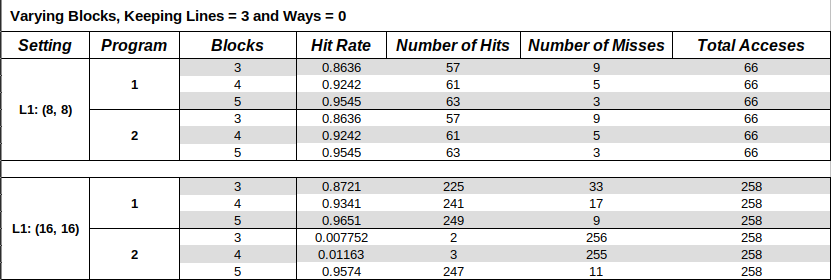
\includegraphics[width=1\textwidth]{1.2.png}
  %\caption{\large Performance Parameters}
  \label{fig:example}
\end{figure}
\noindent
\textbf{\large{Inference :}}\\
\begin{enumerate}[label=\alph*)]
  \item Program 1: Larger block size increases the hit rate due to contiguous memory access.
  \item Program 2: Larger block size enhances hit rate by increasing the chances of the requested word being present in the cache.
\end{enumerate}
\textbf{\large{Note :}}\\
In the latter setting for program 2, the hit rate jumps suddenly due to the huge increase in block size and increased spatial locality.
\smallskip

\subsection{Variation with Ways :}
\begin{figure}[H]
  \centering
  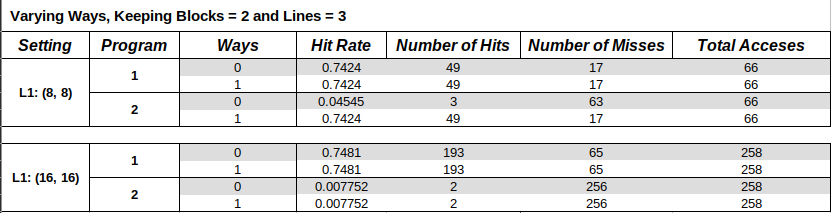
\includegraphics[width=1\textwidth]{1.3.png}
  %\caption{\large Performance Parameters}
  \label{fig:example}
\end{figure}
\noindent
\textbf{\large{Inference :}}\\
\begin{enumerate}[label=\alph*)]
  \item Program 1: The number of ways doesn't significantly affect the hit rate, as once a block is exhausted, it is not accessed again.
  \item Program 2: Increases the hit rate by utilizing data fetched in the past, taking advantage of the temporal locality of the program.
\end{enumerate}
\smallskip

\section{Question 2 :}
\textbf{\large{
Write-policies: Modify programs 1 and 2 to replace “ld x20, 0(x12)” to “sd x20, 0(x12)”. Use the preset cache configuration (32-entry 4-word direct mapped). Run program-1 and program-2 for various combinations of Write-through and Write-back policies (with allocate and without allocate).
}}
\begin{figure}[H]
  \centering
  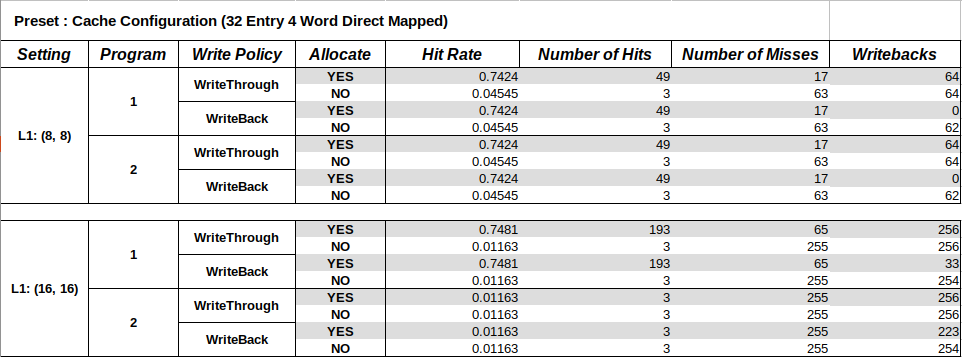
\includegraphics[width=1\textwidth]{2.png}
  %\caption{\large Performance Parameters}
  \label{fig:example}
\end{figure}
\noindent
\textbf{\large{Inference :}}\\
\begin{enumerate}[label=\alph*)]
  \item Program 1: Allocation allowed increases the number of hits compared to when disallowed, regardless of the policy. This is because a block is allocated in the cache on a miss, increasing subsequent hits due to increased spatial locality.
  \item Program 2: In the former setting, the above logic applies. However, in the latter setting, the data is too large to benefit from spatial locality i.e before it can be accessed again it's replaced by another block due to collisions.
\end{enumerate}
\smallskip

\section{Question 3 :}
\textbf{\large{
Associativity: Execute program 3 and vary the following configurations:
\begin{enumerate}
\item[a)]32-entry 4-word direct mapped
\item[b)]32-entry 4-word 2-way set associative
\item[c)]32-entry 4-word fully associative
\end{enumerate}
}}
\begin{figure}[H]
  \centering
  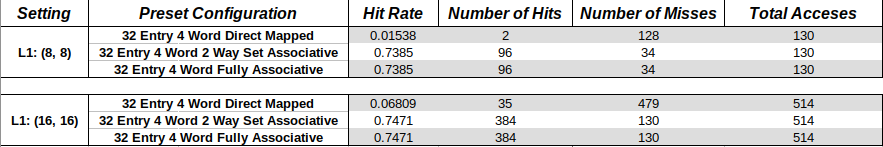
\includegraphics[width=1\textwidth]{3.png}
  %\caption{\large Performance Parameters}
  \label{fig:example}
\end{figure}
\noindent
\textbf{\large{Inference :}}\\
As the data is the same, having more ways would be beneficial, allowing retention of older blocks and possibly taking advantage of any temporal locality the program may have.
\smallskip

\end{document}

